\documentclass[12pt]{article}

\usepackage[paper=letterpaper,margin=2.5cm]{geometry} % Set Margins

%% Math and math fonts
\usepackage{amsmath, amsthm, amssymb, amsfonts}
\usepackage{bbm} % for \mathbbm{1}

% Color
\usepackage{color, xcolor}

% Misc
\usepackage{environ}  % \collect@body in asmmath
\usepackage{graphicx} % \includegraphics options
\usepackage{mdframed} % text boxes
\usepackage{indentfirst} % Indent first paragraph after section header
\usepackage[shortlabels]{enumitem} % Control enumerate items with [(a)]
\usepackage{comment} % Comments
\usepackage{fancyhdr} % Headers and footers

% Tables
\usepackage{array}

% Sub-figures and figure placement
\usepackage{caption}
\usepackage{subcaption}
\usepackage{float} 

% Graphing
\usepackage{pgfplots}
\pgfplotsset{compat=1.17}
\usepackage{tikz}

% Title Placement
\usepackage{titling}
\setlength{\droptitle}{-6em}

% %%%% Theme %%%% % Colors from https://yaleidentity.yale.edu/web
% \definecolor{YaleBlue1}{HTML}{00356b}
% \definecolor{YaleBlue2}{HTML}{286dc0}
% \definecolor{YaleBlue3}{HTML}{63aaff}
% \definecolor{YaleGray1}{HTML}{222222}
% \definecolor{YaleGray2}{HTML}{4a4a4a}
% \definecolor{YaleGray3}{HTML}{978d85}
% \definecolor{YaleGray4}{HTML}{dddddd}
% \definecolor{YaleWhite}{HTML}{f9f9f9}
% \definecolor{YaleGreen}{HTML}{5f712d}
% \definecolor{YaleOrange}{HTML}{bd5319}

%set indent to 
\setlength{\parindent}{0pt}

%for headers 
\pagestyle{fancy}

\lhead{Creel}
\chead{Capital Gains}
\rhead{Nature as Capital}

\title{Section 5 -- The Significance of Capital Gains}
\author{Andie Creel}
\date{March 6rd, 2023}

% Hyper refs
\usepackage{hyperref}
\hypersetup{
    colorlinks=true,
    linkcolor=blue,
    urlcolor  = blue,
    filecolor=magenta,      
    urlcolor=blue,
    citecolor = blue,
    anchorcolor = blue
}

% % Citation management
% \usepackage{natbib}
% \bibliographystyle{agsm}
% \setcitestyle{authordate,open={(},close={)}}

\begin{document}
\maketitle

\section{Introduction}
One of the main lessons from last week is that fishermen aren't stupid. Given that this is true, why do fishermen over-harvest without coordination? What is the market failure that leads to overharvesting, and how can that market failure be internalized?\footnote{Market failure means that one of the core assumptions about competitive markets leading to efficient outcomes is failing. In this case, it's that there is a negative externality. Internalizing that externality means applying a market solution so that an efficient outcome is reached despite a market failure.}\\

When there is no coordination/market intervention, fishermen will over-harvest. This is the tragedy of the commons aka an open access problem. \\

Fishermen do not own the capital (fish) because there are no assigned property rights (everyone can fish as much as they want). This is equivalent to having an infinite discount rate meaning that you don't care about the next time period at all. \textbf{If you don't own capital, you cannot experience capital gains.} Therefore, when fishermen write down their objective function to calculate their optimal amount of harvest, they will not include capital gains. \\

Consider a social planner (\textit{i.e.,} the government) who has the ability to regulate the fishery. The ability to regulate gives the social planner a sense of ownership of the capital (fish). Therefore, \textbf{the social planner does experience the benefit of capital gains. }

\section{Fishermen's Optimization Problem (static solution)}
Note: Static means you only account for one time period.\\

Because fishermen are only optimizing their profit (aka welfare, dividends) their \textbf{objective function} is 

\begin{align}
    \max_h W(h)\\
    W(h)= ph -c(h)
\end{align}

\textbf{Solution form:} An value for $h$ that is only a function of $p$ and the parameters in the cost function. \\

\textbf{Tool to maximize}: Take the derivative and set it equal to zero. Not using a Lagrangian because there is no constraint, not using a Hamiltonian because we're not accounting for capital gains. \\

Optimality condition: 
\begin{align}
    \frac{\partial W}{\partial h} = p - \frac{\partial c}{\partial h} = 0 \label{static_foc}
\end{align}

Solve \ref{static_foc} for $h^\infty(p, \cdot)$.

\section{Social Planner's Optimization Problem (Dynamic Solution)}
Note: Dynamic means you're accounting for multiple time periods \textit{i.e.,} your accounting for intertemporal welfare (\textit{intertemporal welfare} should immediately be causing you to think a Hamiltonian may be the tool of choice). \\

The social planner cares about fishermen's profit (\textit{aka} dividend, welfare) and also \textbf{the capital gains you get from the growth of the stock}. \\

\textbf{Objective Functions:}
\begin{align}
    \max_h W(h) + \lambda \dot s \\
    W(h)= ph -c(h)\\
    \dot s = rs(1 - \frac{s}{K}) - h
\end{align}

\textbf{Solution form:}An value for $h$ that is only a function of $p$ and, the parameters in the cost function, the parameters in the growth rate $\dot s$.\\

\textbf{Tool for maximizing:} The current value you Hamiltonian 
\begin{align}
    H = ph -c(h) + \lambda (rs(1 - \frac{s}{K}) - h)
\end{align}

\textbf{Optimality Conditions: }
\begin{align}
    \frac{\partial H}{\partial h} &= p - \frac{\partial C}{\partial h} - \lambda = 0 \label{FOC_1} \\
    \frac{\partial H}{\partial s} &= ... = \delta \lambda - \dot \lambda \label{FOC_2}
\end{align}
where \ref{FOC_1} is our first optimality condition of a Hamiltonian and \ref{FOC_2} is our second optimality condition of a Hamiltonian (Refer to Section Four Lagrangian vs Hamiltonian notes). \\

\textbf{Finding optimal $h^*$:} If we solve \ref{FOC_1} for $h$, we'll find the socially optimal harvest level. However, it will  be a function of $\lambda$. \\

\textbf{Finding $\lambda$:} We can rearrange \ref{FOC_2} to solve for $\lambda$ which is our Euler equation (refer to week four, natural capital class notes) 
\begin{align}
    \lambda = \frac{\pi_s + \dot \lambda}{\delta - \dot s_s(s)}
\end{align}

and then we can solve for $h^*$!\\

\begin{figure}[htp]
    \centering
    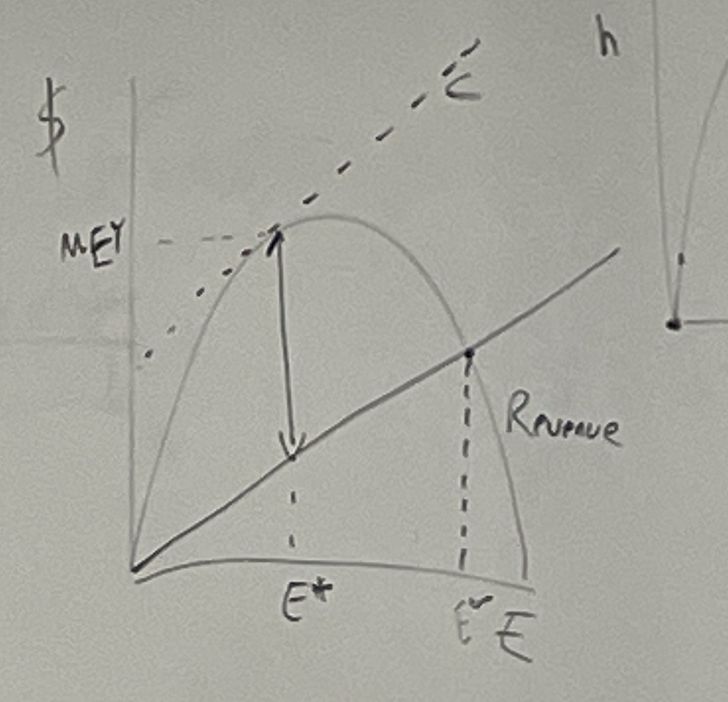
\includegraphics[width=8cm]{Screen Shot 2023-03-01 at 9.38.11 AM.png}
    \caption{We have $h$ on the x-axis instead of E}
    \label{max_econ_yeild}
\end{figure}

\section{Policy Intervention}
If the social planner wanted to impose a market intervention on the fishermen to get them to harvest $h^*$ instead of $h^\infty$, the social planner could impose a tax.\\

The social planner sets the tax equal to the shadow price because the social planner wants the fishermen to account for the marginal value of an additional unit of stock in the fishery (definition of shadow price). This shadow price multiplied by the growth of the stock is the capital gain. 


\subsection{Fishermen's Optimization Problem with Tax}
Now, when the fishermen solve their static problem, their costs have to take into account the tax. Their profit equation is now 
\begin{align}
    \pi = ph - c(h) - \tau h
\end{align}
and so when the fishermen gets his own static FOC it is
\begin{align}
    \frac{\partial \pi}{\partial h} = p - \frac{\partial c}{\partial h}- \tau = 0 \label{FOC_static_tax}
\end{align}
and notice that \ref{FOC_static_tax} is the same as \ref{FOC_1} (because we choose the tax to equal to shadow price $\tau = \lambda$)!! And so our static problem's solution for the optimal $h$ will now be the same as the dynamic problems. 


\section{Connecting $h$ and $E$}

Last week, we saw the Continuous Schaefer Harvest Function
\begin{align}
    h = q E S
    \label{schaefer}
\end{align}
where $q$ is a parameter measuring catch-ability (fraction of population you catch for one unit of effort), $E$ is effort, and $S$ is stock. \\

This is saying that harvest $h$ is a function of effort $E$. We could have plugged this Shaefer harvest function in at the beginning and solved for optimal effort $E$ instead of optimal harvest $h$. Alternatively, if you solved for optimal $h$, you can plug this equation in at the end and solve for $E$ and solve for optimal $E$ at the end. 

\end{document}